%%&program=xelatex
%&encoding=UTF-8 Unicode
% SVN keywords
% $Author$
% $Date$
% $Revision$
% $URL$
\documentclass[a4paper,12pt]{article}      % Comments after  % are ignored
%\usepackage{hyperref}                 % For creating hyperlinks in cross references
%
\usepackage{ifxetex}% for XELATEX, or PDFlatex
\usepackage{ifplatform} 
%
\ifxetex
	\usepackage{polyglossia} \setmainlanguage{portuges}
	\usepackage{fontspec}
	\ifwindows
		\setmainfont[Ligatures=TeX]{Garamond}
		\setsansfont[Ligatures=TeX]{Gill Sans MT}
		\setmonofont[Scale=MatchLowercase]{Courier}
	\fi
	\iflinux
		\setmainfont[Ligatures=TeX]{Linux Libertine O}
		\setsansfont[Ligatures=TeX,Scale=MatchLowercase]{Linux Biolinum}
		\setmonofont[Scale=MatchLowercase]{Courier}
	\fi
	\ifmacosx
	% add settings
	% Use xelatex -no-shell ...
	\fi
	\usepackage{xcolor,graphicx} 
\else
	\usepackage[portuguese]{babel}
	%\usepackage[latin1]{inputenc}
	\usepackage[utf8]{inputenc}
	\usepackage[T1]{fontenc}
	\usepackage{graphics}                 % Packages to allow inclusion of graphics
	\usepackage{color}                    % For creating coloured text and background
\fi

\usepackage{enumitem}
\setlist{nolistsep}
\usepackage{amsmath,amssymb,amsfonts} % Typical maths resource packages

\oddsidemargin 0cm
\evensidemargin 0cm

\pagestyle{myheadings}         % Option to put page headers
                               % Needed \documentclass[a4paper,twoside]{article}
\markboth{{\small \it  Laboratório de Física Experimental Básica}}
{{\small\it MEFT - 1º Sem. 2013/2014} }

\addtolength{\hoffset}{-0.5cm}
\addtolength{\textwidth}{2.5cm}
\addtolength{\topmargin}{-1.5cm}
\addtolength{\textheight}{3cm}

%\textwidth 15.5cm
%\topmargin -1.5cm
\setlength{\parindent}{0pt}
\setlength{\parskip}{1ex  plus  0.5ex  minus  0.2ex}
%\parindent 0.5cm
%\textheight 25cm
%\parskip 1mm


% Math macros
\newcommand{\ud}{\,\mathrm{d}} 
\newcommand{\HRule}{\rule{\linewidth}{0.5mm}}

\author{Prof. Bernardo B. Carvalho} 

%%%%, Bernardo Brotas Carvalho\\bernardo@ipfn.ist.utl.pt} 
\date{ Outubro 2012} 

\begin{document} 

	
\includegraphics[width=0.2\textwidth]{../logo-ist}%\\[1cm]  %%  Logo_IST_color

	\HRule \\[0.5cm]
	{ \huge \sf  \textsc{Velocidade da Luz} }\\[0.4cm] % \bfseries 
%	{ \large \bfseries Determinação Experimental da Carga $q$ do Eletrão }\\
%	{ \large \bfseries Procedimento Experimental}\\
	\HRule \\%[0.5cm]

\section{\sf Introdução}
Em muitas das experiências descritas na literatura para
determinacão da velocidade da luz tem-se utilizado feixes luminosos
modulados que percorrem determinados trajetos de maior ou menor
comprimento, tudo dependendo da forma e frequência da modulação
utilizada. 
No presente trabalho utiliza-se como fonte luminosa um díodo que
emite radiação eletromagnética visível com um comprimento de onda na
zona do vermelho. A tensão aplicada ao díodo emissor é alternada
sinusoidal de frequência $f=50\,MHz$ verificando-se assim que o sinal luminoso
que este emite é Modulado em Amplitute(AM) naquela frequência. 

\begin{equation*}
	\label{eq:f_am}
		s_{diodo}(t) = \underbrace{A_0 \sin ( 2\pi \cdot 50\times 10^6 \, t)}_\text{Amplitude Modulada} \cdot \sin ( 2\pi \cdot f_{luz} \, t)
\end{equation*}

%\section{\sf Introdução}

\section{\sf Base do Método}
No presente trabalho o feixe luminoso proveniente do díodo emissor
é forçado a percorrer um determinado trajeto sendo em seguida detetado
por um foto-díodo receptor (Fig. 1). O sistema de espelhos E, constituído
pelos espelhos E1 e E2, pode deslocar-se ao longo de uma calha graduada,
sendo assim possível variar o comprimento do trajeto do raio luminoso. Os
sinais de amplitude impostos ao emissor e captados no receptor são aplicados\footnote{Depois de uma deteção \emph{homodínica}, em que a frequência modulada é desviada $f_{}=50\, MHz -50.050\, MHz = 50\,kHz$. Esta operação permite a utilização deum osciloscopio de banda estreita.} 
aos canais de um osciloscópio funcionando no modo “XY”.

O sinal visualizado no osciloscópio é uma figura de Lissajous e normalmente uma elipse de equação geral:
\begin{equation}
	\label{eq:elipse}
	\sin^2 \delta = \frac{x^2}{x_0^2} + \frac{y^2}{y_0^2} - \frac{2y\,x}{y_0\,x_0} \cos  \delta
\end{equation}

\begin{figure}
	[!htb]  \centering 
	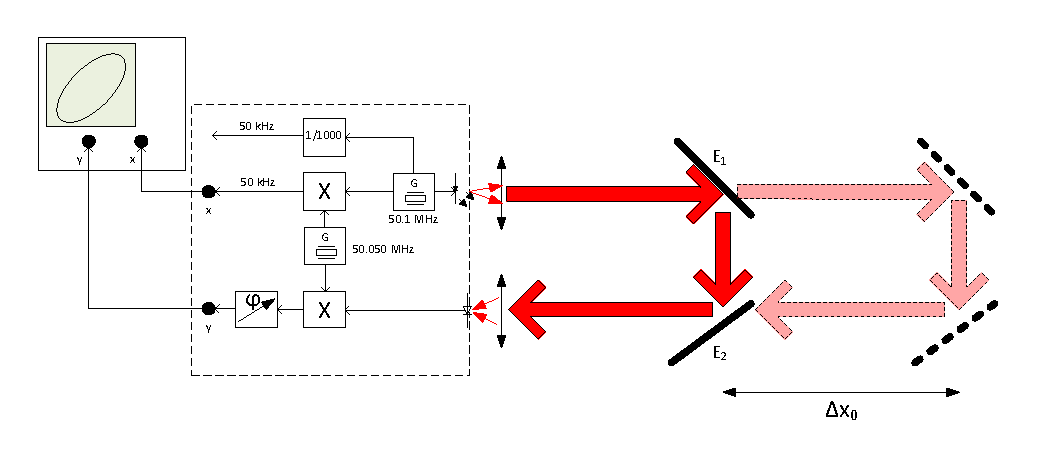
\includegraphics[width=0.8\textwidth]{Vel_esquema}
	\caption{Montagem para determinar a Velocidade da Luz. \label{fig:Montagem}} 
\end{figure}

Sendo $x(t)$ o sinal proveniente do emissor,  $x_0$  a sua amplitude,  $y(t)$ o sinal
proveniente do recetor, $y_0$ a sua ampliıude e $\delta$ a desfazagem entre os dois
sınais. A elipse pode degenerar em retas quando os dois sinais estiverem
em fase $\delta = 2n\,\pi$  ou em oposição de fase $\delta = (2n+1)\,\pi$. 

\subsection{\sf Velocidade da Luz no ar}
Neste trabalho a
velocidade da luz é calculada a partir da determinação do comprimento do
caminho suplemenıar que a luz tem de percorrer para que se passe de uma
situação em que os sinais estão em oposição de fase à situação contígua de
fase ($2\,\Delta\,x$). Assim a luz percorre esse comprimento suplementar num intervalo de
tempo que é igual a metade do periodo ($T/2$) do sinal modulante ($T=1/50\,MHz= 20\,ns$). 

\begin{figure}
	[!htb]  \centering 
	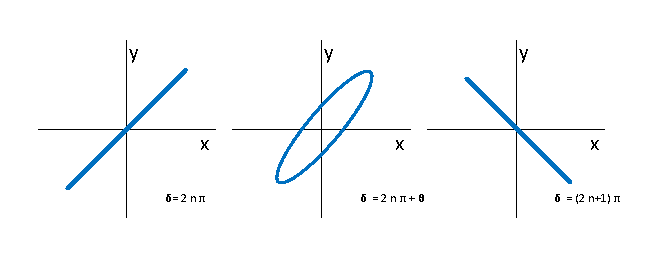
\includegraphics[width=0.8\textwidth]{osci_fase}
	\caption{Figuras de Lissajous observadas no osciloscópio. \label{fig:fase}} 
\end{figure}

No ar teremos:
\begin{equation}
	\label{eq:vc}
	c_{ar} = \frac{2\,\Delta x_0}{T/2} 
\end{equation}

\subsection{\sf Velocidade da Luz em meios sólidos e líquidos}
Neste trabalho será também determınada a velocidade da
luz em  mais dois meios materiais uma resina e a água. 
A partir dos valores obtidos 
será também possível calcular o índice de refração da resina e da água em
relação ao ar. Assim o índice de refração de
a um meio material $1$ em relação a um meio material $0$
 para um dado comprimento de onda pode ser definido como a relação entre as velocidades de propagação da luz no meio 
 $0$ e no meio $1$ \footnote{Esta definição só é válida se as condutividades dos meios $0$ e $1$ forem nulas.}
 
 
 \begin{equation}
	\label{eq:index}
	n= \frac{c_0}{c_1}  = \frac{\frac{1}{\sqrt{\varepsilon_0 \, \mu_0}} }{\frac{1}{\sqrt{\varepsilon_1 \, \mu_1}} } =
		\sqrt{\frac{\varepsilon_1 \, \mu_1}{\varepsilon_0 \, \mu_0}} = \sqrt{\varepsilon_r \, \mu_r}
\end{equation}

Nesta expressão $\varepsilon_0$, $\varepsilon_1$ e $\varepsilon_r$   e  $\mu_0$, $\mu_1$, e $\mu_r$ são as constantes dielétricas  as permeabilidades magnéticas respetivamente do meio $0$, do meio $1$ e relativa $(\varepsilon_1= \varepsilon_r\, \varepsilon_0)$.

\begin{figure}[h!tb]  
	\centering 
	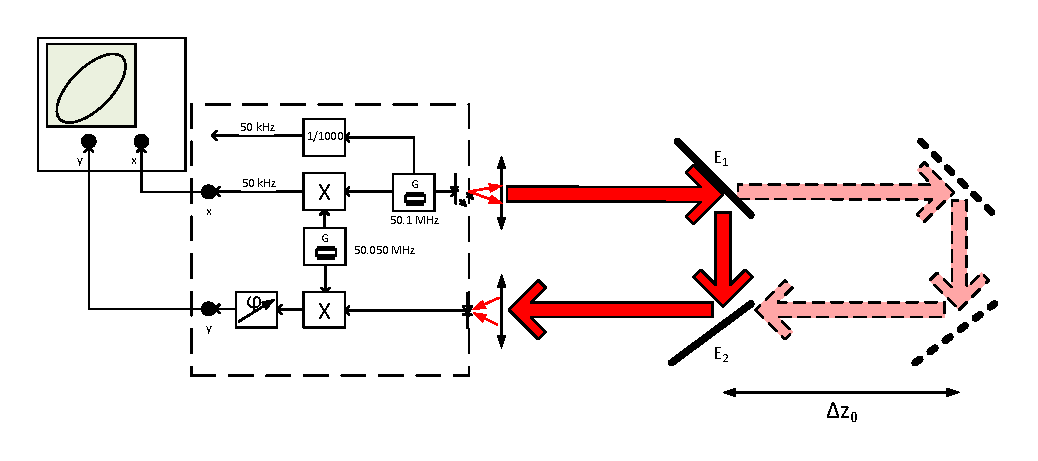
\includegraphics[width=0.8\textwidth]{Vel_esquema_bloco}
	\caption{Montagem para determinar a Velocidade da Luz. \label{fig:Montagem_bloco}} 
\end{figure}

Se no percurso do feixe luminoso interpormos um bloco de material sólido ou líquido transparente 
 de comprimento $l_B$ (Figura \ref{fig:Montagem_bloco}) então a expressão  (\ref{eq:vc}) pode ser generalizada em:

\begin{equation}
	\label{eq:vc_bloco}
	{T/2}  = \frac{2\,\Delta x_1 - l_B}{c_{ar}}  +  \frac{l_B}{c_{B}}
\end{equation}

De onde se pode pode extrair a velocidade $c_{1}$. 
Também se pode obter  o indíce de refração $n_{B}$ a partir de (\ref{eq:vc}) e (\ref{eq:index}).

\begin{align}
	\label{eq:n_bloco}
	{T/2}  = \frac{2\,\Delta x_0}{c_{ar}}  &=  \frac{2\,\Delta x_1 }{c_{ar}} -   \frac{l_B}{c_{ar}}  +  \frac{l_B}{c_{B}} \nonumber \\ 
	\frac{2\,(\Delta x_0- \Delta x_1 )}{c_{ar}}  &= -   \frac{l_B}{c_{ar}}  +  \frac{l_B}{c_{B}} \nonumber \\
	\frac{2\,(\Delta x_0- \Delta x_1 )}{l_B} &= -1 +  \frac{c_{ar}}{c_{B}} \nonumber \\
	n_{B} &= 1 +  \frac{2\,(\Delta x_0- \Delta x_1 )}{l_B}
\end{align}

\newpage
\section{\sf Protocolo Experimental}
\subsection{\sf Material utilizado}

\begin{enumerate}
\setlength{\itemsep}{0mm}
\item Unidade de emissão de luz (díodo emissor) e de recepção (díodo receptor)
[amplitude modulada por um sinal de frequência $50\,MHz$] 
\item Duas lentes plano-cilindrícas
\item Conjunto de dois espelhos planos para inversão do sentido de propagação da luz 
\item Calha graduada (até 1.50m em 0.5cm) 
\item Bloco de vidro acrílico transparente 
\item Dois tubos com cerca de 1 metro de comprimento para conter água ou ar. 
\item Osciloscópio de dois canais a funcionar em modo XY
\end{enumerate}

\subsection{\sf Procedimento Experimental}
\subsubsection{\sf Regulação da montagem}
 
Comece por verificar se a montagem está regulada. Teste a evolução da forma da mancha 
luminosa ao longo do percurso óptico usando um alvo difusor (por exemplo, papel vegetal) e 
verifique que está centrada com a lente receptora e com o orifício que permite iluminar o 
díodo receptor. Ajuste os parafusos dos espelhos de forma a maximizar a amplitude do sinal 
recebido.
Coloque os espelhos na posição de zero da escala e, rodando o botão que modifica 
continuamente a diferença de fase entre os dois sinais, coloque-os em fase. 

\subsubsection{\sf Velocidade de propagação da luz no ar}
Desloque os espelhos sobre a calha e observe a modificação da figura no ecrã do 
osciloscópio, em particular, nas posições que correspondem aos sinais recebidos estarem 
desfasados de π/2 (quadratura) e em oposição de fase. Para esta última situação registe a 
posição dos espelhos e o domínio espacial para o qual os sinais parecem estar ainda em 
oposição de fase. Repita a medida pelo menos duas vezes (cada observador). 
Calcule a velocidade de propagação da luz no ar e os desvios à precisão e à exatidão. 

\subsubsection{\sf Velocidade de propagação da luz no vidro acrílico}
Verifique de novo se no zero da escala os sinais estão em fase. Coloque o bloco de vidro 
acrílico no feixe incidente de modo que entre perpendicularmente às faces e faça o percurso 
mais longo no vidro acrílico. Meça a posição (e a incerteza correspondente) dos espelhos tal 
que os dois sinais detetados estejam em oposição em fase. Repita a medida pelo menos 
duas vezes (cada observador).
Calcule o valor da velocidade obtido para o vidro acrílico e os desvios à precisão e à 
exatidão. Calcule o índice de refração do vidro acrílico.

\subsubsection{\sf Velocidade de propagação da luz na água}
Verifique de novo que no zero da escala os sinais estão em fase. Coloque o tubo vazio de 
água nos suportes de modo que o feixe incidente entre perpendicularmente às faces.
Registe a posição dos espelhos que produz um sinal em oposição de fase com o incidente. 
Repita estas medidas para o tubo cheio de água. 
Calcule o valor da velocidade obtida para a água e os desvios à precisão e à exatidão. 
Calcule o índice de refração da água. 
Comente criticamente a precisão do valor da velocidade de propagação da luz obtida nos 
diferentes meios.
\end{document} 